\section{Lösungsansätze in Big-Data Umgebungen}

Im Big-Data Umfeld wurden die Grenzen relationaler Datenbanken früh erkannt und an entsprechenden Lösungsansätzen gearbeitet. Als größtes Hindernis wurde Distanz zum relationalen Datenmodell und deren strikten Einschränkungen geschaffen.

\subsection{NoSQL - flexibel und skalierbar}

Der Begriff NoSQL beschreibt eine Familie von Datenbanken welche sich von dem traditionellen relationalen Datenbankmodell distanzieren. In der Literatur wird dieser typischerweise interpretiert mit \enquote{not only SQL}, entgegen der intuitive Übersetzung \enquote{kein SQL}. Der Unterschied zu relationalen Datenbanken liegt in der Art und Weise wie Daten gespeichert werden. Statt der Bindung an ein fest definiertes Datenschema, sind NoSQL-Datenbanken flexibel. Es wird im Allgemeinen zwischen vier Datenmodellen unterschieden:

\begin{enumerate}[nosep]
    \item \textbf{Schlüssel-Wert-Datenbanken} speichern Daten als Paarungen aus einem eindeutigen Schlüssel und einem zugehörigen Wert. Der Schlüssel dient zur Identifizierung des Werts, ähnlich wie ein Primärschlüssel in RDBMS. \footcite[S. 2]{wangSQLVsNoSQL2017}
    \item \textbf{Spaltenorientierte Datenbanken} speichern Daten in Spaltenfamilien statt, wie bei RDBMS üblich, in Zeilen. Zusammengehörige Daten werden somit aggregiert gespeichert und ermöglichen hohe Skalierbarkeit durch Verteiliung der unterschiedlichen Spaltenfamilien auf verschiedene Knoten. 
    \item \textbf{Dokumentorientierte Datenbanken} verwalten Daten in flexiblen, hierachisch strukturierten Dokumenten, meist im JSON-Format. Jedes Dokument kann eine unterschiedliche Struktur aufweisen, wodurch dynamische und variable Datenmodelle untersützt werden.
    \item \textbf{Graphdatenbanken} speichern Daten als Knoten und deren Beziehungen als Kanten. Vernetzte Datenstrukturen, bei denen die Beziehungen zischen Datenelementen im Vordergrund stehen, können in Graphdatenbanken effizient abgebildet werden.
\end{enumerate}

Die ersten drei Datenbanktypen unterscheiden sich in ihrer Art, stark von den Graphdatenbanken. Fowler schlägt daher die Teilung der NoSQL-Familie  in zwei übergreifende Kategorien vor: Die Aggregat-orientierten Datenbanken, speichern zusammengehörige gemeinsam ab. Hier ist der Unterschied zu relationalen Datenbanken erkennbar, wo zusamenhängende Daten meist durch die Normalisierung auseinandergerissen werden. Graphdatenbanken hingegen, sind spezialisiert auf die noch stärkere Verteilung von Daten welche nicht im direkten Zusammenhang zueinander stehen, sondern lediglich in Bestimmten Situationen oder Anwendung in Verbindung oder Beziehung zueinander stehen. \footcite{fowlerAggregateOrientedDatabase2012}

\subsection{Zurück zu SQL - NewSQL}
%\subsection{Zurück zu (New)SQL}

Das zweite Kapitel dieser Arbeit behandelte bereits ausführlich die Limitierungen und Grenzen relationaler Datenbanken, insbesondere in den domänenspezifischen Anforderungen von BigData. Nichts, desto trotz scheinen relationale Datenbanken immernoch der Standard zu sein, trotz aller Nachteile. Der Grund hierfür liegt aller Vermutung nach in der Abfragesprache SQL. Die universelle Datenbankübergreifende Sprache, basierend auf dem relationalen Modell, scheint der Vorteil zu sein, der sämtliche Nachteile in den Schatten stellt. Die chaotische, Abfragesituation bei NoSQL bei welcher jede Datenbankimplementierung eigenen Syntax und Grammatik verwendet wird hierbei nicht hilfreich gewesen sein. 

In den letzten Jahren wurden die Froderungen nach einer erneuten Vereinheitlichung der Abfragesprachen lauter. Neue Datenbanken sollten nun, sämtliche Vorteile der NoSQL Ära mit mit den Vorteilen der SQL Äre verbinden. Dieser Ansatz wird heute als NewSQL bezeichnet, und beschreibt den Trend zurück zu SQL oder SQL ähnlicher Abfragesprachen. Die Autoren \textit{Stonebreaker und Pavlo} beschreiben diese Situation treffend in ihrem Artikel aus mit dem Titel \textit{\enquote{What Goes Around Comes Around... And Around...}} \footcite{stonebrakerWhatGoesComes2024}.

\newpage

\subsection{Fallstudie: Datenbankarchitektur eines Online-Shops}

In der Vergangenheit war die Wahl der Datenbank unkompliziert - Es musste lediglich die Entscheidung getroffen werden auf welches RDBMS gesetzt werden soll. Doch mit dem Aufkommen der NoSQL Datenbanken wurde diese Entscheidung deutlich schwieriger. Nicht musste von nun an zwischen zwei Datenbankmodellen entschieden werden, sondern auch innerhalb von NoSQL gibt es verschiedene Datenbanktypen optimiert für unterschiedliche Anwendungsseznarien. Auch die Erfahrung der Entwickler spielt nun eine Rolle, da man sich nicht mehr auf die universellen SQL-Kenntnisse verlassen kann. Doch die resultierenden Vorteile kompensierten den erhöhten Aufwand. Während für die allermeisten Anwendungen mit strukturierten Daten, relationale Datenbanken die beste Wahl darstellen, gibt es Anwendungsseznarien wo eine andere Wahl sinnvoller ist. Abbildung 1 zeigt eine beispielhafte Datenbankarchitektur eines großen Online-Shops wie z.B. Amazon.de.

\begin{figure}[H]
    \centering
    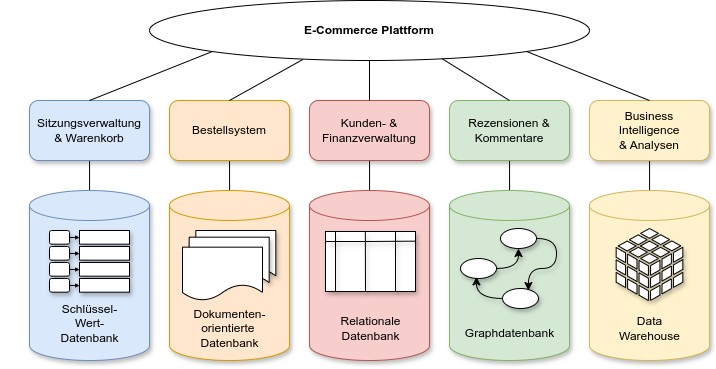
\includegraphics[width=\textwidth]{online-shop-db-architecture.png}
    \caption{Datenbankarchitektur eines Online-Shops, angelehnt an \cite{donofrioBigDataAnalytics2021}.}
    % \footcite[S. 7]{meierWerkzeugeDigitalenWirtschaft2018}
\end{figure}

Erkennbar ist, das für alle Funktionen verschiedene Datenbankmodelle gewählt wurden. Für die Verwaltung der Nutzersessions und Warenkörbe könnte eine simple Schlüssel-Wert-Datenbank sinnvoll sein. Für das Bestellsystem, ist die Flexibilität und Skalierbarkeit von NoSQL ebenfalls wichtig, weshalb ein Dokumentspeicher in Betracht zu ziehen ist. Für die Verwaltung der Benutzeraccounts sind die ACID eigenschaften relationaler Datenbanken besonders wichtig. Bei den Produktrezensionen und Kommentaren liegen stark vernetzte Daten vor, weshalb eine Graphdatenbank sinnvoll erscheint. Auch für die Business Intelligence möchte man das passende System verwenden, hier kommt Beispielweise ein Data Warehouse basiernd auf einer Spaltenfamiliendatenbank in Frage.

Polyglot Persitstance !!! 